\documentclass{beamer}
\usepackage{amsmath, amssymb, amsthm}
\usepackage{booktabs, graphicx, geometry}
\usepackage{setspace, cite}
\usepackage{listings, xcolor}
\usepackage{verbatim, pgfplotstable}

\lstset{
  language=Python,
  basicstyle=\ttfamily\footnotesize,
  keywordstyle=\color{blue}\bfseries,
  commentstyle=\color{gray}\itshape,
  stringstyle=\color{orange},
  numbers=left,
  numberstyle=\tiny\color{gray},
  breaklines=true,
  frame=single,
  backgroundcolor=\color{black!5}
}

\usetheme[progressbar=frametitle]{metropolis}
%\usecolortheme{spruce}
\usepackage{appendixnumberbeamer}
\usepackage{metropolisbrown} % Don't forget to load this!
\setbeamertemplate{navigation symbols}{}

%title pagee
\title{Coggins' Search Method}
\subtitle{}
\author{\bf{Samuel Dark}}
\date{\today}

\begin{document}

\maketitle


%Introduction
\section{Introduction}
\begin{frame}[allowframebreaks]{Introduction}
\begin{itemize}

\item Search methods for unconstrained optimization fall into two broad
categories \cite{odekunle2009}:
\begin{enumerate}
    \item \textbf{Direct search methods}: require only objective
    function evaluations; no derivatives are needed.
    \item \textbf{Descent methods}: exploit gradient information to
    determine search directions.
\end{enumerate}

\item The Coggins search method is a direct optimization technique
that iteratively searches for an optimum by adaptively
adjusting step sizes.
\item It is an interpolation-based approach that requires few function
evaluations and uses unequally spaced points to bracket the minimum,
followed by successive quadratic approximations resulting in rapid
convergence \cite{bamigbola2004}. 
 \end{itemize}
\end{frame}




%Coggins method
\section{Coggins' Search Mehtod}
  \begin{frame}[allowframebreaks]{Algorithm}
   The classical Coggins method is a combination of the single-variable
search technique proposed by Davies et al.\ and Powell
\cite{bamigbola2004}. It is designed to optimize an objective
function of a \textit{single} variable $x \in \mathbb{R}$.

\subsection{Algorithm}

The algorithm proceeds as follows \cite{odekunle2009}:

\begin{enumerate}
    \item A starting point $x_0$ is chosen and the objective function
    $f(x_0)$ is evaluated.

    \item The variable is incremented by a step size $\Delta x$ and
    $f(x_0 + \Delta x)$ is evaluated.
    \begin{itemize}
        \item If a function improvement is obtained, the step size is
        \textbf{doubled} for the next evaluation.
        \item If no improvement is obtained on the first step, the
        direction is \textbf{reversed} and the next point is located
        at a distance $\Delta x$ from the starting point.
    \end{itemize}

    \item This bracketing continues until a local optimum is
    straddled, yielding three points around the optimum $(x_{k-2},\hspace{0.1cm} x_{k-1}, \hspace{0.1cm} x_{k})$. 
    
    \item An additional point $x_{k+1}$ is then located at:
    \begin{equation}
        x_{k+1} = x_{k-1} + \frac{\Delta x}{2}
    \end{equation}
    where $\Delta x$ is the current step size. The best three
    points are retained, say $(x_1, x_2, x_3)$.

    \item The \textbf{quadratic interpolation} is used to iteratively to find the optimum. The optimum $x^*$ is located by setting
    $\frac{df}{dx} = 0$, giving:
    \begin{equation}
        x^* = \frac{
            (x_2^2 - x_3^2)f(x_1) +
            (x_3^2 - x_1^2)f(x_2) +
            (x_1^2 - x_2^2)f(x_3)
        }{
            2\bigl[(x_2 - x_3)f(x_1) +
                   (x_3 - x_1)f(x_2) +
                   (x_1 - x_2)f(x_3)\bigr]
        }
        \label{eq:quad_interp}
    \end{equation}

    \item The objective function at $x^*$ is compared with the best
    previous point subject to a convergence criterion:
    \begin{equation}
        |f(x^*) - f(x_{\text{best}})| \leq \varepsilon
    \end{equation}

    \item If the criterion is satisfied, the procedure stops.
    Otherwise, the worst point is replaced by $x^*$, a new quadratic
    surface is fitted, and steps 4--6 are repeated.
\end{enumerate}
 
\end{frame}



%Algorithm
\section{Algorithm Implementation}
\begin{frame}{Algorithm Implementation}
  The Coggins method was implemented using Python.
  The implementation follows three stages:

  \bigskip
  \begin{enumerate}
    \item \textbf{Define} $f(x)$
    \item \textbf{Bracketing Phase}: locate three points straddling
      the minimum using step-doubling and $x_{k+1} = x_b +
      \frac{\Delta x}{2}$
    \item \textbf{Quadratic Fitting}: repeatedly fit a quadratic
      to the three best points and compute $x^*$ until
      $|f(x^*_{\text{new}}) - f(x^*_{\text{best}})| \leq
      \varepsilon_{\lim}$
  \end{enumerate}
\end{frame}

\begin{frame}[fragile]{Stage 1: Objective Function}
  We define the test function to be minimized:
  \[
    f(x) = x^4 - 14x^3 + 60x^2 - 70x, \qquad x_0 = 0,
    \quad \Delta x = 1
  \]
  where $x_0$ is our intial point and $\Delta x$ is the step-size.
  \begin{lstlisting}
def f(x):
    return x**4 - 14*x**3 + 60*x**2 - 70*x
\end{lstlisting}

  \bigskip
  This function has two local minima. Cogins' method will find the nearest minimum.
  
\end{frame}

\begin{frame}[fragile, allowframebreaks]{Stage 2: Bracketing and Step-Doubling}
\begin{itemize}
    \item Starting at $x_0 = 0, \quad f(x_0) $ is evaluated.
    \begin{lstlisting}
    def bracket_minimum(func, x0, delta=1.0):
    xa = x0
    fa = func(xa)
    \end{lstlisting}
    \item  We step forward and evaluate $f(x_0+\Delta x)$.
    \begin{lstlisting}
    xb = xa + delta
    fb = func(xb)
    \end{lstlisting}
    \item Upon improvement, we continuously doubled the step size and evaluated the function at each new point until $f(x_k) \geq f(x_{k-1})$, confirming the minimum is straddled.\vspace{0.5cm}

The loop ends when the bracketed points $(x_{k-2}, x_{k-1}, x_{k})$ satisfy the condition; \quad $f(x_{k-2}) \geq f(x_{k-1})$ and
  $f(x_k) \geq f(x_{k-1})$ \vspace{0.5cm}

    \item After confirming the straddle, we locate an additional point $x_{k+1}=x_{k-1}+\Delta x/2$ to improve accuracy
    \begin{lstlisting}
         x_k1 = xb + delta / 2.0
    f_k1 = func(x_k1)
    \end{lstlisting}
    The best three out points out of the four is bracketed. 
\end{itemize}
\begin{verbatim}

  Bracketing from x0 = 0.0,  initial delta = 1.0

  Point                     x           f(x)  Action
  ──────────────────────────────────────────────────────────────
  xa                 0.000000       0.000000  starting point
  xb                 1.000000     -23.000000  first step
  xc (iter 1)        3.000000      33.000000  delta doubled to 2.00000

  Straddle confirmed: f(xc) >= f(xb).
  Minimum lies between xa = 0.0000 and xc = 3.0000.

  x_(k+1)            2.000000       4.000000  fourth point: xb + delta/2 = 1.0000 + 1.0000

  Best three points retained (sorted by x):
  ──────────────────────────────────────────────────────────────
  x1                 0.000000       0.000000
  x2                 1.000000     -23.000000  <- lowest f
  x3                 2.000000       4.000000
  ──────────────────────────────────────────────────────────────
  Straddle check:  f(x1) >= f(x2): True,  f(x3) >= f(x2): True
\end{verbatim}

The best three points now tightly straddle the optimum
  and are ready for quadratic fitting
\end{frame}

\begin{frame}[fragile, ]{Stage 3: Quadratic fitting}
    With $x_1, x_2, x_3$ straddling the optimum, we compute
  $x^*$ \cite{odekunle2009}
  \begin{lstlisting}
      def quadratic_minimum(x1, x2, x3, f1, f2, f3):
    numerator = (
        (x2**2 - x3**2) * f1 +
        (x3**2 - x1**2) * f2 +
        (x1**2 - x2**2) * f3
    )
    denominator = 2.0 * (
        (x2 - x3) * f1 +
        (x3 - x1) * f2 +
        (x1 - x2) * f3
    )

    return numerator / denominator
  \end{lstlisting}
   We iterate until $|f(x^*_{\text{new}}) -
  f(x^*_{\text{best}})| \leq \varepsilon$: where we chose $\varepsilon =10^{-6}$
\end{frame}

\begin{frame}{Quadratic Fitting (output)}
    \begin{verbatim}
Quadratic Refinement
  ──────────────────────────────────────────────────────────────
  Iter            x*           f(x*)          |Δf|
  ──────────────────────────────────────────────────────────────
     1      0.960000      -23.440957      4.41e-01
     2      0.824477      -24.311850      8.71e-01
     3      0.769577      -24.365640      5.38e-02
     4      0.779899      -24.369572      3.93e-03
     5      0.780977      -24.369601      2.97e-05
     6      0.780882      -24.369602      2.68e-07
  ──────────────────────────────────────────────────────────────
  Converged after 6 iteration(s).
  ──────────────────────────────────────────────────────────────
  Minimum at  x*  =  0.78088230
  f(x*)           =  -24.36960157
  ──────────────────────────────────────────────────────────────

\end{verbatim}

\end{frame}

\begin{frame}{Algorithm Impllementation Results}
  \begin{figure}
    \centering
    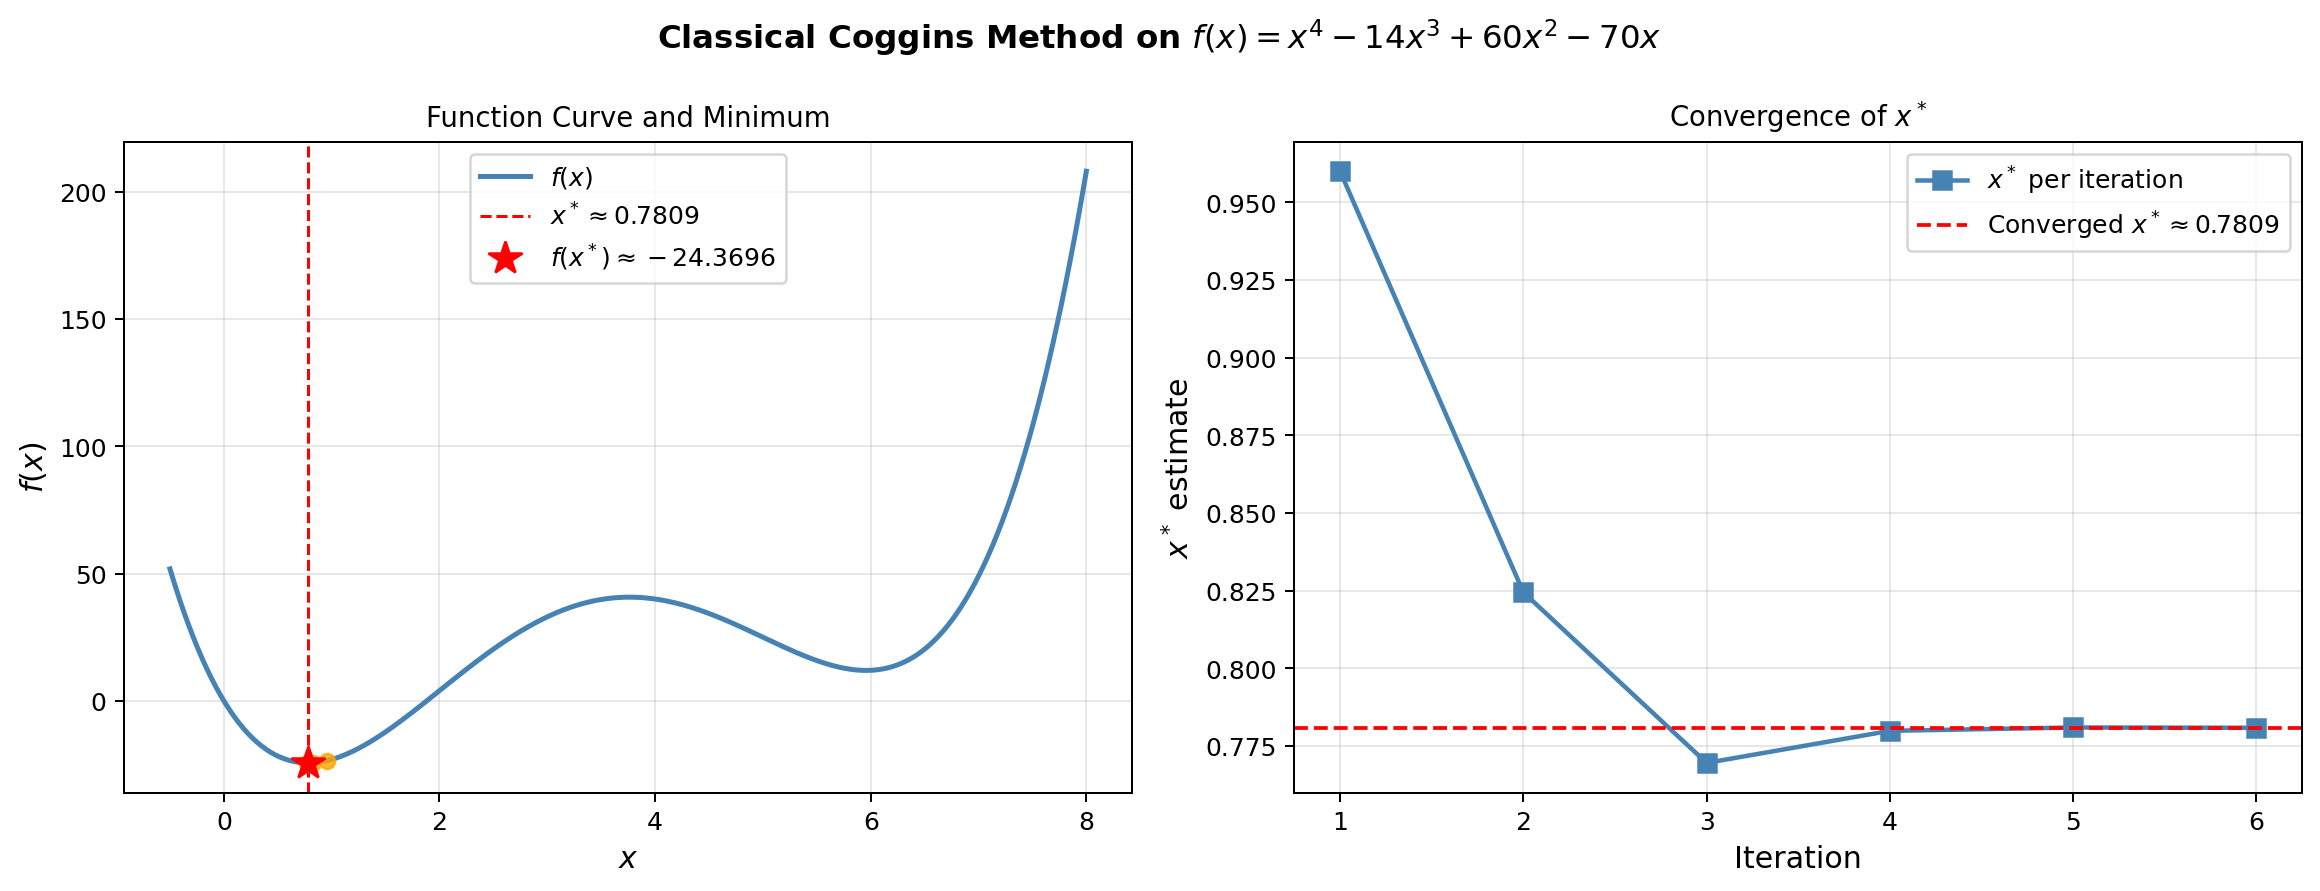
\includegraphics[width=\linewidth]{coggins_quartic.png}
    \caption{Left: $f(x)$ with minimum found at
    $x^* \approx 0.78$, $f(x^*) \approx -24.37$.\\
    Right: convergence of $x^*$ across iterations.}
  \end{figure}
\end{frame}

\begin{frame}{Verification}
  We verify $x^* \approx 0.78$ is a minimum using calculus:

  \bigskip
  First order condition:
  \[
    f'(x) = 4x^3 - 42x^2 + 120x - 70 = 0 \quad
    \text{has a root near } x \approx 0.78 \checkmark
  \]

  \bigskip
  Second order condition:
  \[
    f''(x) = 12x^2 - 84x + 120
  \]
  \[
    f''(0.78) = 12(0.78)^2 - 84(0.78) + 120
    = 61.78 > 0 \checkmark
  \]

  \bigskip
  Since $f''(x^*) > 0$, the curve is concave at $x^*$,
  confirming a \textbf{local minimum}.
\end{frame}


\begin{frame}{Key Features}

The classical Coggins method is efficient in that it:
 \begin{itemize}
    \item requires relatively few function evaluations.
    \item uses \textit{unequally spaced} points to bracket the
    minimum.
    \item achieves rapid convergence through successive quadratic
    approximations.
\end{itemize}

 \end{frame}

 
\section{Conclusion}
\begin{frame}[allowframebreaks]{Conclusion}
\begin{itemize}
       \item Coggin's Search Method is a useful technique for step-size determination.
      \item It transforms multidimensional optimization into a one-dimensional search problem.
\item The method improves efficiency through interpolation.
\end{itemize}
\end{frame}

\section{References}

\bibliographystyle{plain}
\bibliography{myref}

\end{document}